% *** LaTeX-mal for labrapporter i fysikk, v.14.08.2017 ***

% Dette er et eksempel på et LaTeX-dokument, og du kan bruke dette som et utgangspunkt for din egen rapport. Merk at for å kunne kompilere dokumentet uten feil, må du også laste ned filen pendel-oppdatert.pdf.
%
% Her i starten og videre nedover i teksten under har vi lagt inn en god del linjer som starter med tegnet "%". Disse linjene er kommentarer og synes ikke i det ferdige dokumentet. Vi kan også sette inn et kommentartegn midt på en linje. Alt som kommer fÞr tegnet brukes da i kompileringen, mens resten av linja er en kommentar. 
%
% Kildefilen (.tex-filen) begynner alltid med et "preabmle". Her setter man opp innstillingene som brukes av kompilatoren til å utforme det ferdige dokumentet. Selve dokumentet begynner ikke fÞr vi skriver \begin{document}.
%
% Dokumentasjon for alle pakker finnes på CTAN (http://www.ctan.org/)

%%%%%%%%%%%%%%%%%%%%%%%%%%%%%%%%%%%%%
% Preamble
%%%%%%%%%%%%%%%%%%%%%%%%%%%%%%%%%%%%%

\documentclass[5p,sort&compress]{elsarticle}		
% 5p gir 2 kolonner pr side. 1p gir 1 kolonne pr side.
% Valget sort&compress gjÞr at referansen [1,2,3] settes som [1-3]. 
% Andre innstillinger for "klassen" elsarticle finnes i dokumentasjonen på CTAN (http://www.ctan.org/pkg/elsarticle)

% Klassen elsarticle er laget for bruk i engelskspråklige tiksskrift. I blokken under bruker vi litt lavnivå TeX-magi for å redefinere bunnteksten på tittelsiden. Ikke bekymre deg for denne biten med kode, det som kommer lengere nede i dokumentet er lettere å forstå!
\makeatletter
\def\ps@pprintTitle{%
 \let\@oddhead\@empty
 \let\@evenhead\@empty
 \def\@oddfoot{\footnotesize\itshape
       Levert til Fredrik Nicolai Krohg	% Bytt ut "Veileder" med navnet på veilederen din!
       \hfill\today}%
 \let\@evenfoot\@oddfoot}
\makeatother

% Encoding for input i tex-filen og encoding for output i pdf-filen
\usepackage[utf8]{inputenc}
\usepackage[T1]{fontenc}
\usepackage{textcomp}
\usepackage{amsmath}
\usepackage{gensymb}

\usepackage{siunitx}


\usepackage{placeins} %FloatBarrier

% Last inn en font-pakke. Her bruker vi standard-fonten til LaTeX. 
\usepackage{lmodern}

% LaTeX gjÞr mye av typografien for deg, blant annet orddeling ved linjeskift og automatisk utfylling av endel tekst. For å kunne gjÞre dette må kompilatoren vite hvilket språk dokumentet er skrevet på. 
\usepackage[norsk]{babel}
\usepackage[fixlanguage]{babelbib}
% Til tross for at vi har fortalt kompilatoren at vi skriver på norsk må vi fortelle den eksplisitt at vi Þnsker at seksjonen "abstract" skal kalles "sammendrag"
\renewenvironment{abstract}{\global\setbox\absbox=\vbox\bgroup
\hsize=\textwidth\def\baselinestretch{1}%
\noindent\unskip\textbf{Sammendrag}
\par\medskip\noindent\unskip\ignorespaces}
{\egroup}

% Mikrotypografiske optimeringer
\usepackage[babel=true]{microtype}

% AMS-utvidelsene for å håndtere matematikk
\usepackage{amsmath}
\usepackage{amssymb}
\usepackage{bm}

% Måltall og enheter er spesielle typografiske dyr som reguleres av strenge regler. For å gjÞre det enklere å håndtere tall og enheter på riktig måte bruker vi pakken siunitx.
\usepackage{siunitx}
% Vi tilpasser standardinstillingene til pakken til norske regler. 
\sisetup{
exponent-product = \cdot,
output-decimal-marker  =  {,}, % Pass på å endre desimalskilletegnet til punktum om du skriver på engelsk!
separate-uncertainty = true,
per-mode = symbol,
group-digits = false,
}

% Figurer og tabeller
\usepackage{graphicx} % Denne pakken er standard for å kunne laste inn figurfiler med ulike formater
% LÞsne opp på de alt for strenge standardinstillingene for plassering av figurer og tabeller (floats) i LaTeX-kjernen
\renewcommand{\topfraction}{.85}
\renewcommand{\bottomfraction}{.7}
\renewcommand{\textfraction}{.15}
\renewcommand{\floatpagefraction}{.66}
\setcounter{topnumber}{3}
\setcounter{bottomnumber}{2}
\setcounter{totalnumber}{10}
\usepackage{flafter} % For å plassere floats i PDFen fÞrste sted LaTeX tillater etter det punktet de er definert i TeX-filen. Om du definerer figuren i TeX-filen rett etter at du refererer til den for fÞrste gang vil denne pakken sÞrge for at de fleste floats havner på greie steder
\usepackage{booktabs} % Denne pakken gir tilgang på endel ekstra kommandoer som legger til rette for god skikk og bruk i tabellformatering.
\usepackage{multirow}
\usepackage[font=small,labelfont=bf]{caption}	% Justering av LaTeX standarder for figurtekst og tabelltekst.

% Hyperreferanser
\usepackage[colorlinks=true,allcolors=blue]{hyperref}
% Noen av navnene for autoreferanser mangler på norsk, så vi ordner opp i det.
\addto\extrasnorsk{%
\def\figureautorefname{figur}%
\def\tableautorefname{tabell}%
\def\sectionautorefname{avsnitt}%
\def\subsectionautorefname{underavsnitt}%
}
% Vi endrer fonten som brukes for URLer til den vanlige tekstfonten.
\urlstyle{same}

%%%%%%%%%%%%%%%%%%%%%%%%%%%%%%%%%%%%%
% Selve dokumentet
%%%%%%%%%%%%%%%%%%%%%%%%%%%%%%%%%%%%%

\begin{document}

% I "front matter" angir vi formalia knyttet til dokumentet -- tittel, forfatter, tilknytning og sammendrag
\begin{frontmatter}

\title{Rullefriksjon mellom metallkule og hardplast}

% I forfatterlisten legger vi inn "ikke-brytende" mellomrom etter initialene
\author[fysikk]{A. Aurlien}
\author[fysikk]{M. Storebø}
\author[fysikk]{P. B. Hove}
\author[fysikk]{T. Berntsen}

\address[fysikk]{Institutt for fysikk, Norges teknisk-naturvitenskapelige universitet, 7491 Trondheim.}

\begin{abstract}
En måte å estimere rullefriksjonskoeffisienten mellom stål og hardplast er å la en stålkule oscillere i en sirkelbane av hardplast og måle utslaget fra likevektposisjonen over tid.
Friksjonskoeffisienten er forholdet mellom friksjonskraft og normalkraft, og ved noen tilnærminger gjort i grunnlag i lite krumning, er proporsjonal med tapet i utslaget fra likevektsposisjonen til kulen.
Rullefrikssjonskoeffisienten ble estimert analytisk til $\mu_E = (1,40 \pm 0,03) \cdot 10^{-3}$ og ved numerisk løsning av systemet ble rullefriksjonskoeffisienten estimert til $\mu_N = 1,653 \cdot 10^{-3}$. Dette er i samme størrelsesorden som friksjonskoeffisienter for tilsvarende systemer.
Avviket mellom numerisk beregnet- og analytisk beregnet friksjonskoeffisient kan ikke forklares med tilnærmingene som er gjort av modellen, og ser ut til å være et samspill av flere effekter som er utelatt i den teoretiske modellen. 
\end{abstract}

\end{frontmatter}


\section{Introduksjon}
Ideelt sett ville en kule som ruller frem og tilbake i en halvsirkel gått like langt opp for hver gang. Det vil si at den ikke ville mistet energi på grunn av friksjon. I virkeligheten er ikke dette tilfellet. En kjent verdi av rullefriksjonskoeffisienten for stål mot stål er mellom 0,0010 og 0,0015 ~\cite{friksjonskoeffisienter}. I denne rapporten skal rullefriksjonskoeffisienten mellom stål og hardplast estimeres ved å utføre et eksperiment hvor en stålkule oscillerer frem og tilbake på en sirkelbane av hardplast.

Gjennom historien har rullefriksjon vært et hinder for transport. Helt siden hjulet ble oppfunnet har mennesker prøvd å redusere rullefriksjonen for å effektivisere fremkomstmidler. Det å kjenne rullefriksjonskoeffisienter mellom forskjellige materialer er derfor viktig for å bestemme hvilke materialer som bør brukes i konstruksjonen av slike fremkomstmidler.  



\section{Teori}
Newtons andre lov beskriver sammenhengen mellom kreftene som virker på et legeme, legemets masse og legemets akselerasjon. 
\begin{equation}
\sum{\vec{F}} = m \vec{a},
\label{eq:Newtons Andre Lov} 
\end{equation}
hvor \textit{m} er legemets masse og $\vec{a}$ er legemes akselerasjon. For et legeme som beveger seg i en sirkelbane kan en dekomponere kreftene som virker på legemet i x- og y-retning. Positiv x-retning er definert tangensielt på sirkelbanen i retning mot klokken. Positiv y-retning er definert normalt på rulleretning, mot sentrum av sirkelen, slik som i \autoref{fig:skraplan}. Newtons andre lov normalt blir da

\begin{equation}
\sum{F_y} = F_{N} - F_{G_y} = m a_y,
\end{equation}
hvor $F_y$ er summen av kreftene i y-retning, $F_{G_y}$ er tyngdens komponent normalt på planet, definert ved $F_{G_y} = mg \cos\alpha(x)$, $F_N$ er er normalkraften, m er legemets masse og $a_y$ er legemets akselerasjon i y-retning og $g$ er tyngdens gravitasjonskonstant. Dersom legemet ruller, og en ser bort fra luftmotstand, blir Newtons andre lov, i x-retning, gitt ved
\begin{equation}
\sum{F_x} = F_{G_x} - F_{R} - F_{F} = m a_x, \\
\end{equation}
hvor $F_{G_x}$ er tyngdekraftens komponent tangensielt på planet, definert ved $F_{G_x} = mg\cos(\alpha)$.  $F_{F}$ er statisk friksjonskraft som skaper rulling, som er definert ved $F_{F} = \frac{I_{0}\ddot{x}}{r^2} $, der $I_{0}$ er kulens treghetsmoment og $r$ er radiusen til legemet.
 $F_{R}$ er rullefriksjon definert ved $F_{R} = \mu F_{N}$. $\alpha$ er vinkelen mellom tangentplanet på banen og horisontalaksen. $\alpha$ kan beskrives som en funksjon av posisjonen. 


\FloatBarrier
\begin{figure}[h!]
\centering
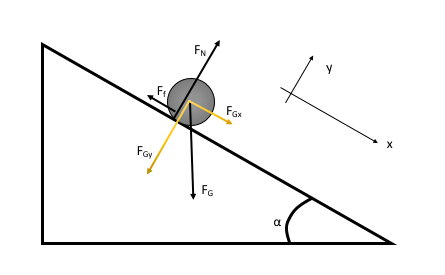
\includegraphics[width=0.4\textwidth]{Lysbilde1.png}

\caption{Krefter som påvirker et legeme, dekomponert i x og y retning i henhold til rulleretning, i en infinitesimal del av sirkelbanen. $F_F$ er friksjonskraften, $F_G$ er gravitasjonskraften, $F_G_y$ er gravitasjonskraftens komponent i y-retning, $F_G_x$ gravitasjonskraftens komponent i x-retning, $F_N$ er normalkraften og $\alpha$ er vinkelen mellom tangenten til sirkelbanen og horisontallinjen.}
\label{fig:skraplan} % Som med ligningen er dette det interne navnet på figuren.
\end{figure}
\FloatBarrier

Ved å anta $\omega=vr$, hvor $\omega$ er vinkelhastigheten til legemet, altså ingen sluring, får en at 
\begin{equation}
    \ddot{x} = K \left(g sin(\alpha (x)) - \mu \left(g cos(\alpha (x)) + \frac{v^2}{R}\right)  \frac{\dot{x}}{|\dot{x}|}\right),
    \label{diffing}
\end{equation}
der $K = \frac{1}{(1+\frac{I_{0}}{mr^2})}$. $\frac{\dot{x}}{|\dot{x}|}$ er normalisert fartsvektor til legemet. 
For små vinkler gir tilnærmingen $ \sin\alpha \approx \frac{x}{R} $ og $\cos\alpha \approx 1$  små avvik, hvor \textit{R} er radius til sirkelbanen. Disse antagelsene er vist i \autoref{fig:halvsirkel}. 
Ved små hastigheter og stor sirkelradius vil $\frac{v^2}{R}$ være neglisjerbar.
Dersom en kun ser på en halv periode vil $\frac{\dot{x}}{|\dot{x}|} = 1$ Da løses \eqref{diffing} for x slik
\begin{equation}
\label{eq:Posisjon av tid}
x(t) = (x_{0} + R\mu)cos(\sigma t)-R\mu,
\end{equation}
der $\sigma^2=\frac{K}{R}$. 

Fra eksperimentelle måledata kan $\mu$ beregnes. Ved å benytte at et legeme når sin største x-verdi ved $cos(\sigma t) = -1$ får vi at høyeste x-verdi er gitt ved
$$x\left( \frac{T}{2} \right) = -x_0 - 2R\mu,$$
hvor T er svingeperioden. For hver periode vil utslag fra likevektsposisjonen synke med $4R\mu$. 
Velger en å beregne $\mu$ ved å måle tapet av utslag fra likevektsposisjonen over fire perioder vil $\mu$ være gitt ved

\begin{equation}
\label{eq:Utrykk for my}
\mu = \frac{\Delta x}{16R},
\end{equation}
der $$\Delta x = x(4T) - x_{0},$$ og $x_{0}$ er initialposisjon.
\FloatBarrier
\begin{figure}[h!] 
\centering
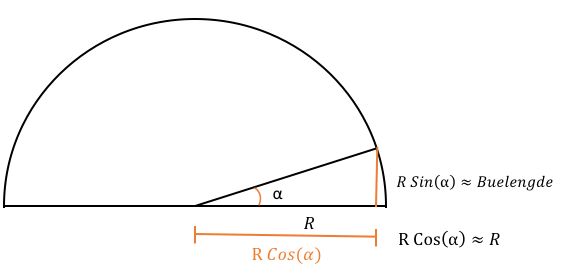
\includegraphics[width=0.4\textwidth]{halvny.png}

\caption{Representasjon av sinus og cosinus for små vinkler. $\alpha$ er vinkelen og $R$ er radien.}
\label{fig:halvsirkel} % Som med ligningen er dette det interne navnet på figuren.
\end{figure}
\FloatBarrier

Målte størrelser vil alltid begrenses av nøyaktigheten i målingen. Skal en se på resultatene i slutten av et eksperiment er det derfor viktig å utføre en usikkerhetsanalyse for å kunne avgjøre om resultatet er nøyaktig eller om resultatet har for stor usikkerhet til at resultatet faktisk kan brukes.
I beregning av en verdi hvor flere målte størrelser inngår, kan Gauss feilforplantningslov gi et mål på den totale usikkerheten til verdien som skal beregnes. For å kunne bruke ligningen for Gauss feilforplantningslov må gjennomsnittet og usikkerheten til hver av de målte størrelsene være kjent.

Å finne standardavviket er første steg for å regne ut usikkerheten til en gjennomsnittsverdi.
Standardavvik \cite{Usikkerhet} er gitt ved
\begin{equation}
\label{eq:Standardavvik}
\delta{x}=\sqrt{\frac{1}{N-1}\sum\limits_{i=1}^N (x_{i}-\overline{x})^2},
\end{equation}
hvor $\overline{x}$ er gjennomsnittet, \textit{N} er antall datapunkt og $x_i$ er hvert datapunkt.
Usikkerheten til en gjennomsnittverdi \cite{Usikkerhet} er gitt av
\begin{equation}
\label{eq:Standardfeil}
\delta\overline{x} = \frac{\delta x}{\sqrt{N}},
\end{equation}
og kalles standardfeilen.
 Gauss feilforplantingslov \cite{Usikkerhet} er gitt ved:  
\begin{equation}
\label{eq:Gauss feilforplantningslov}
\delta f = \sqrt{(\frac{\partial f}{\partial x}\cdot\delta x)^2+(\frac{\partial f}{\partial y}\cdot\delta y)^2 + ...} .
\end{equation}
Her er $\delta f$ usikkerheten ved en funksjon, f er funksjonen, x og y er variable som inngår i funksjonen.

Radien til en sirkel kan finnes fra følgende ligning gitt et punkt på nedre halvdel av sirkelbanen (se  \autoref{fig:Radien}):
\begin{equation}
\label{eq:Sirkelradius}
R = \frac {c^2+h^2}{2h},
\end{equation}
der c er minste avstanden fra punktet på sirkelbanen til linjen mellom sirkelens mittpunkt og bunnpunkt.
\FloatBarrier
\begin{figure}[h!] 
\centering
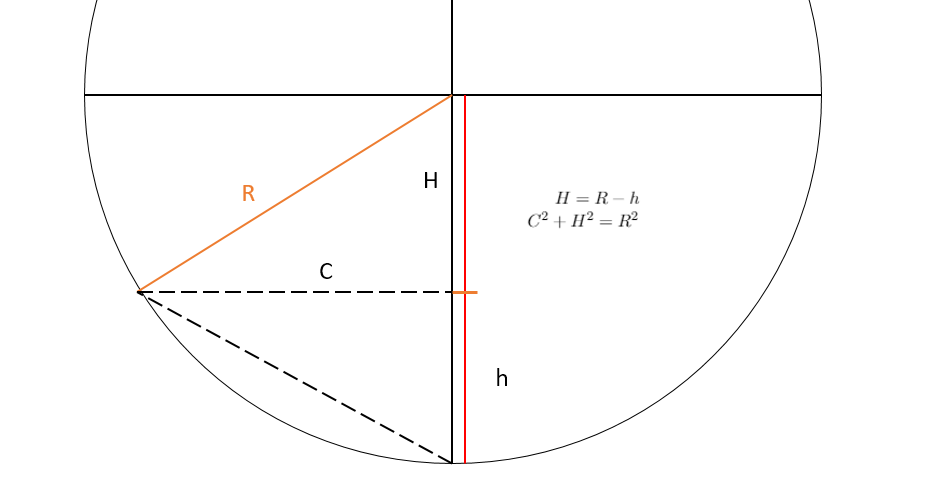
\includegraphics[width=0.4\textwidth]{Rapport/Figurfikset.png}
\caption{Figurer illustrerer sammenhengen mellom høyde over bunnpunkt og avstand fra null punkt. $R$ er radius, $C$ er minste avstand fra punkt på banen til linjen mellom sirkelens mittpunkt og bunnpunkt, $H$ er avstand til normalen $C$ og $h = R - H.$}
\label{fig:Radien} % Som med ligningen er dette det interne navnet på figuren.
\end{figure}
\FloatBarrier


\section{Eksperimentell metode}
Eksperimentets startoppsett vises i \autoref{fig:pendel}. Eksperimentet utføres på en sirkelbane av hardplast. Banen har syv holdepunkter plassert en fast lengde, $20,0 \hspace{0,5mm}\mathrm{cm} \pm 0,1 \hspace{0,5mm}\mathrm{cm}$, fra hverandre for å holde sirkelbanen. Høyden til hvert holdepunkt beregnes med ligning \eqref{eq:Sirkelradius}, der utgangspunktet er at de ytterste holdepunktene er satt til $5,0 \hspace{0,5mm}\mathrm{cm} \pm 0,1 \hspace{0,5mm}\mathrm{cm}$ og er $60,0 \hspace{0,5mm}\mathrm{cm} \pm 0,1 \hspace{0,5mm}\mathrm{cm}$ fra nullpunkt i x-retning. Et høyhastighetskamera blir satt opp foran banene slik at filmen får samme perspektiv som i figur \autoref{fig:pendel}.

Eksperimentet utføres ved at en stålkule slippes fra et fast startpunkt. Kulen ligger på banen og blir holdt i ro av en linjal. Linjalen blir tatt bort vertikalt. En meterstokk er plassert foran sirkelbanen for kalibrering av avstand på filmen.
Kulen ruller i fem perioder. Videre blir filmen fra kameraet analysert i et dataprogram, Tracker~\cite{Tracker}, som gir data for kulens posisjon ved en gitt tid. Analyse av filmen startes etter det er gått en periode.
Dette eksperimentet blir utført ti ganger.

Det ble også utført en numerisk løsning av ligning \eqref{diffing} som beskriver rullebevegelsen. 
Ligningen ble løst numerisk med Eulers metode ~\cite{Euler}. Det ble brukt tidssteg 0,001s, da lavere tidsteg gir neglisjerbar endring i løsningen. Det simuleres over 4 perioder der banen som brukes i simuleringen er beskrevet av et polynom. Polynomet finnes ved interpolasjon av datapunkter fra Tracker. Polynomet er plottet i \autoref{fig:poly}. 

\begin{figure}[h!] 
\centering
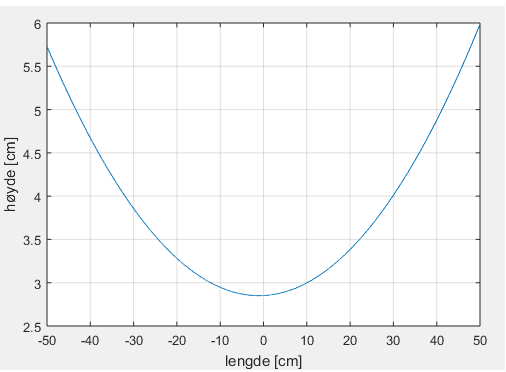
\includegraphics[width=0.4\textwidth]{Rapport/polynomFiksa.png}
\caption{Plot av polynomet som beskriver banen det simulueres over i beregningen av $\mu_N$. x-aksen er utstrekningen til banen og y-aksen er høyden til banen.}
\label{fig:poly} % Som med ligningen er dette det interne navnet på figuren.
\end{figure}
I simuleringen settes startfarten til 0 og utgangsposisjonen blir satt til snittet av eksperimentell verdi etter en periode.
Ved å tilpasse den numeriske løsningen til eksperimentelle start og sluttverdier blir den numeriske løsningen for $\mu$ beregnet. 
\FloatBarrier
\begin{figure}[h!] 
\centering
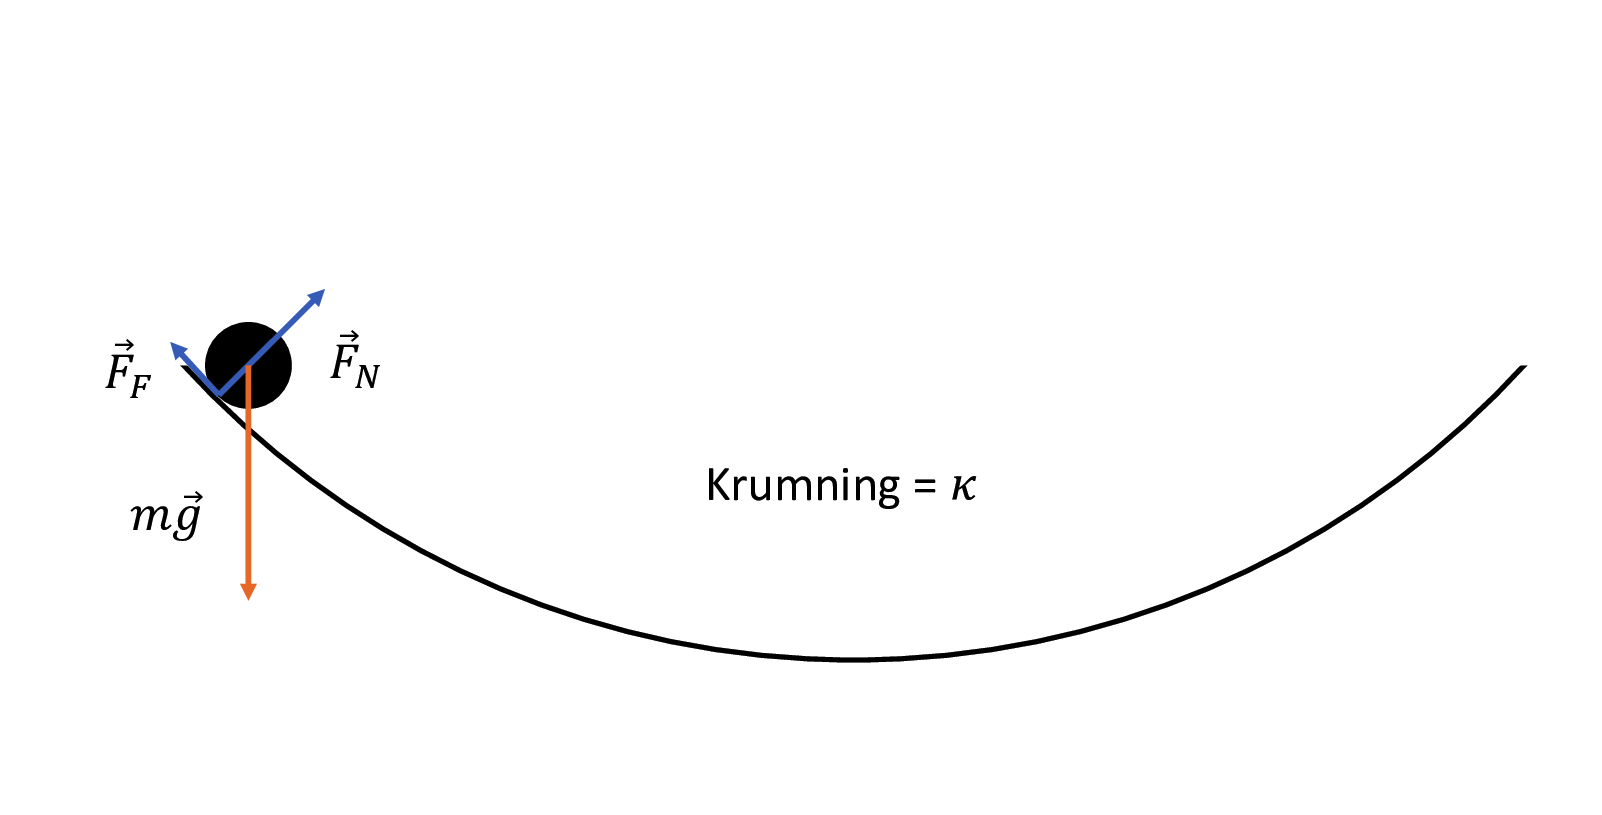
\includegraphics[width=0.4\textwidth]{Figur_til_lab.png}

\caption{Startoppsett av eksperimentet med påvirkende krefter.}
$\kappa$ er krumningen til sirkelbanen, $m$ er kulens masse, $g$ er tyngdekraftens gravitasjonskonstant, $F_F$ er friksjonkraften og $F_N$ er normalkraften.
\label{fig:pendel} % Som med ligningen er dette det interne navnet på figuren.
\end{figure}
\FloatBarrier

\section{Resultater}
Lengden og høyden til ytterste feste på sirkelbanen (i forhold til bunnpunkt på sirkelbanen) ble hhv. målt til $60,0 \hspace{0,5mm}\mathrm{cm} \pm 0,1 \hspace{0,5mm}\mathrm{cm}$ og $5,0 \hspace{0,5mm}\mathrm{cm} \pm 0,1 \hspace{0,5mm}\mathrm{cm}$ der usikkerheten er basert på avlesningsnøyaktighet.
Radien til sirkelen ble beregnet til $363\hspace{0,5mm}\mathrm{cm} \pm 7\hspace{0,5mm}\mathrm{cm}$ ved bruk av ligning \eqref{eq:Sirkelradius}, der usikkerheten ble beregnet ved bruk av Gauss Feilforplantningslov \eqref{eq:Gauss feilforplantningslov}. Gjennomsnittet til $\Delta x$ er lik $8,14 \hspace{0,5mm}\mathrm{cm}$ og ble beregnet med måledataene fra analysen Tracker. 
Den tilhørende standardfeil er $\delta x = 0,05 \hspace{0,5mm}\mathrm{cm},$ beregnet med ligning \eqref{eq:Standardfeil}.
%\vspace{2mm}
Dette gir følgende verdi for eksperimentell rullefriksjonskoeffisient: $\mu_{E} = (1,40\pm 0,03) \cdot 10^{-3}$\\ beregnet ved ligning \eqref{eq:Utrykk for my}. Gauss feilforplantingslov \eqref{eq:Gauss feilforplantningslov} er brukt på ligning \eqref{eq:Utrykk for my} og gir usikkerheten til $\mu_E$ er $\pm0,03\cdot 10^{-3}$. Det vil si at usikkerhet i friksjonskoeffisienten er ≈ $\pm 2,1\%$.

Den numeriske løsningen av systemet tilnærmes eksperimentelle måledata  med fire siffer nøyaktighet, da blir $\mu_N = 1,653 \cdot 10^{-3}$. \autoref{fig:numerisklosning} viser horisontal posisjon plottet mot tid, der $\mu$ er satt slik at den numeriske løsningen har samme verdi etter fire perioder som eksperimentell data. 

\FloatBarrier
\begin{figure}[h!] 
\centering
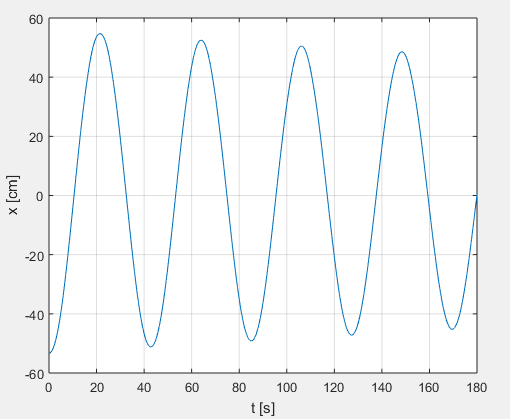
\includegraphics[width=0.4\textwidth]{Rapport/losningnumerik.png}

\caption{Numerisk løsning plottet horisontal posisjon mot tid. Posisjon i cm, tid i sekunder.}
\label{fig:numerisklosning}
\end{figure}
\FloatBarrier


\section{Diskusjon}
En kjent verdi av rullefriksjonskoeffisienten for stål mot stål er mellom 0,0010 og 0,0015~\cite{friksjonskoeffisienter}. Da stål er hardere enn hardplast forventes det at friksjonskoeffisienten for stålkule mot hardplast er høyere enn dette, men i samme størrelsesorden. Fra eksperimentelle verdier ble rullefriksjonskoeffisienten for stål mot hardplast beregnet til $(1,40 \pm 0,03)\cdot10^{-3}$.
Ved å finne $\mu$ slik at numerisk løsning ble mest mulig lik eksperimentell måledata blir $\mu_N = 1,653 \cdot 10^{-3}$. Disse verdiene er rimelige i henhold til forventet resultat. 

Det ble gjort en antagelse om null luftmotstand og null sluring. Ved inspeksjon av høyhastighetsvideo bekreftes det at det er null sluring. Luftmotstand virker som en bremsende kraft og ved lave hastigheter kan luftmotstanden være neglisjerbar. I dette forsøket var rullefriksjonen så liten at luftmotstand kan spille en ikke-neglisjerbar rolle i bremsing av kulen. Derfor vil en friksjonskoeffisient beregnet ved en antagelse om null luftmotstand være for høy i forhold til den faktiske verdien. 

For å bergene $\mu_E$ antas det at $F_N = mg\cos{\alpha}$ basert på at $mg\cos{\alpha} >> \frac{v^2}{R}$. I tilfellet hvor $\frac{v^2}{R}$ utgjør størst relativ verdi utgjør det kun $\sim 1,5 \%$ av $mg\cos{\alpha}$. Da $\frac{v^2}{R}$ neglisjeres får $\mu_E$ en høyere verdi. Det antas også at $\sin{\alpha} = \alpha$ slik at $\sin{\alpha} = \frac{x}{R}$. I ytterpunktene er vinkelutslaget $\sim \ang{10}$ da blir $\frac{\sin{\alpha}}{\alpha} = 0,9952$. Altså vil kulen bevege seg noe lengre enn antatt og antagelsen øker $\mu_E$. Samtidig vil $cos(\sigma t)$ fra ligning \eqref{eq:Posisjon av tid} være større enn antatt, som medfører at $\mu_E$ blir mindre.

Usikkerheten i $\mu_E$ er beregnet ut i fra usikkerheten til radiusen og usikkerheten til $\Delta x$. Det er bidraget fra usikkerheten til radiusen som står for det meste av den totale usikkerheten.

$\mu_N$ er utenfor usikkerheten i $\mu_E$.
Systematiske målefeil kan ikke stå for hele differansen, ei heller antagelser gjort for å løse systemet analytisk da antakelsene medfører mindre avvik. Dette kan skyldes andre feilkilder som ikke er tatt hensyn til.

Dette gjelder for eksempel usikkerhet fra Tracker. Fra rådataene kan en se at dataene er skalert ned, fordi kulen sin distanse i x-retning blir redusert med nesten halvparten av total reduksjon på første runde. Det ble ikke målt startposisjon med Tracker, da dette var vanskelig å få til, men når det antas en konstant prosentvis reduksjon, så kan en rekne startposisjonen til 55-56cm. Kulen ble sluppet fra en avstand på 60cm som betyr at det er en nedskalering på rundt 8$\%$. Dette medfører samme skalering i $\Delta x$ og medfører at $\mu_E$ er for lav i forhold til den faktiske verdien. % Bruk direkte på my som vi har komt fram til, så vert den "nye" myen 1.52

\section{Konklusjon}
Ved å la en stålkule oscillere i en sirkelbane av hardplast ble rullefriksjonskoeffisienten mellom stålkulen og hardplast beregnet til $(1,40 \pm 0,03) \cdot 10^{-3}$. Det er i samme størrelsesorden som antatt.

Systemet ble modellert og løst numerisk. Friksjonskoeffisienten som gjorde modellen tilsvarende rullebevegelsen til kulen ble $\mu_N = 1,653 \cdot 10^{-3}$.

Avviket mellom numerisk beregnet- og eksperimentelt beregnet friksjonskoeffisient kan ikke forklares med målefeil eller antagelsene som ble gjort i eksperimentell modell, da antagelsene bidrar til mindre avvik. Avviket kan skyldes feilkilder som ikke er tatt stilling til. Det er ikke foretatt en detaljert undersøkelse av disse feilkildene.


% Her kommer referanselisten
\begingroup
\begin{center}
\rule{2cm}{.4pt} % Vi markerer starten på referanselisten med en horisontal strek
\end{center}
\makeatletter
\@beginparpenalty=10000 % Vi setter en høy straff for kompilatoren om den setter inn et sideskift mellom streken og starten på referanselisten.
\makeatother
\bibliographystyle{babunsrt}
\bibliography{thomas}
\endgroup

\end{document}